\section{El grupo de las trenzas.}\label{grupotrenzas}
Hemos visto una definición que nos permite saber cuándo dos trenzas son equivalentes, pero es demasiado general como para poder llevarla a la práctica. En esta sección vamos a hacer un estudio más profundo de la teoría de trenzas. Para ello tenemos que empezar viendo que el conjunto ${B}_{n}$, dotado del producto de trenzas que veremos a continuación, tiene estructura de grupo no abeliano.

\begin{center}
     \subsection{Estructura de grupo no abeliano:}
\end{center}

\textbf{\underline{Definición 2.2:}}\label{defpro}\\
Sean las trenzas $\beta$, $\beta' \in \mathscr{B}_{n}$. Definimos su \textbf{producto} $\beta \beta'$ como la n-trenza que se crea al unir los extremos finales de las cadenas de $\beta$ con los extremos iniciales de las cadenas de $\beta'$.\\

En la figura \ref{grupo0} se puede ver un ejemplo del producto de dos trenzas: la trenza (c) es el producto de las trenzas (a) y (b).\\
   \begin{figure}[h!]
   	\centering
   	\subfigure[$\sigma3^{-1}\sigma1$]{
\includegraphics[width=5.5cm]{itrenzas/1c1.png}}
   	\subfigure[$\sigma2\sigma3$]{
\includegraphics[width=5.5cm]{itrenzas/1c2.png}}
   	\space
   	\subfigure[$\sigma3^{-1}\sigma1\sigma2\sigma3$]{
\includegraphics[width=5cm]{itrenzas/1c3.png}}  	
   	\caption{Producto trenzas}
   	\label{grupo0} 
   \end{figure}

\begin{pro}\label{prod1}
	Sean las trenzas $\beta1$, $\beta1'$, $\beta2$, $\beta2' \in \mathscr{B}_{n}$ verificando las equivalencias $\beta1 \sim \beta1'$ y $\beta2 \sim \beta2'$. Entonces se verifica la equivalencia $\beta1\beta2 \sim \beta1'\beta2'$.
	\begin{proof}
		Por hipótesis tenemos $\beta1 \sim \beta1'$ y $\beta2 \sim \beta2'$. Por la definición \ref{defequi} sabemos que existen las secuencias de trenzas equivalentes tales que: 
		\begin{center}
			$ \beta1 = \beta1_{0} \rightarrow \beta1_{1} \rightarrow ... \rightarrow \beta1_{m}=\beta1'$ 
		\end{center}
		\begin{center}
			$ \beta2 = \beta2_{0} \rightarrow \beta2_{1} \rightarrow ... \rightarrow \beta2_{m}=\beta2'$ 
		\end{center}
		Mediante la primera igualdad tenemos 
		\begin{center}
			$ \beta1\beta2 = \beta1_{0}\beta2 \rightarrow \beta1_{1}\beta2 \rightarrow ... \rightarrow \beta1_{m}\beta2=\beta1'\beta2$ luego $ \beta1\beta2 \sim \beta1'\beta2$.
		\end{center}
		Mediante la segunda igualdad tenemos
		\begin{center}
			$ \beta1'\beta2 = \beta1'\beta2_{0} \rightarrow \beta1'\beta2_{1} \rightarrow ... \rightarrow \beta1'\beta2_{m}=\beta1'\beta2'$ 
			luego $ \beta1'\beta2 \sim \beta1'\beta2'$.
		\end{center}
		Por la transitividad de la equivalencia de trenzas se tiene que
\begin{center}
			 $  \beta1\beta2 \sim \beta1'\beta2 \sim \beta1'\beta2'$	
\end{center}	
				
	\end{proof}
\end{pro}

   \begin{figure}[h!]
   	\centering
   	\subfigure[$\sigma3^{-1}\sigma2^{-1}\sigma3^{-1}$]{
\includegraphics[width=3.4cm]{itrenzas/3c1.png}}
   	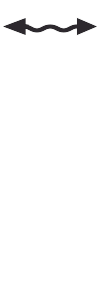
\includegraphics[width=1.2cm]{itrenzas/flechac.png}
   	\subfigure[$\sigma2^{-1}\sigma3^{-1}\sigma2^{-1}$]{
\includegraphics[width=3.6cm]{itrenzas/3c2.png}}
   	\subfigure[$\sigma3^{-1}\sigma1\sigma3^{-1}$]{
\includegraphics[width=3.6cm]{itrenzas/3c3.png}}
   	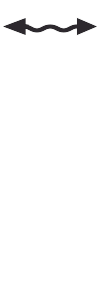
\includegraphics[width=1.2cm]{itrenzas/flechac.png}
   	\subfigure[$\sigma1\sigma3^{-1}\sigma3^{-1}$]{
\includegraphics[width=3.1cm]{itrenzas/3c4.png}}

	\subfigure[$\sigma3^{-1}\sigma2^{-1}\sigma3^{-1}\sigma3^{-1}\sigma1\sigma3^{-1}$]{
\includegraphics[width=4cm]{itrenzas/3c5.png}}
	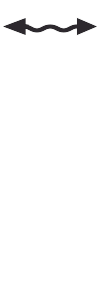
\includegraphics[width=1.5cm]{itrenzas/flechac.png}
	\subfigure[$\sigma2^{-1}\sigma3^{-1}\sigma2^{-1}\sigma1\sigma3^{-1}\sigma3^{-1}$]{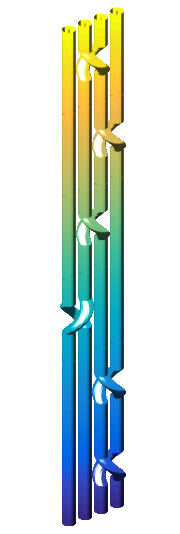
\includegraphics[width=3.2cm]{itrenzas/3c6.png}}   	
   	\caption{Equivalencia producto}
   	\label{grupo1} 
   \end{figure}
   
   Veamos el ejemplo de la figura \ref{grupo1}: Las trenzas (a) y (b) son equivalentes luego la parte superior de las trenzas (e) y (f) es equivalente. Las trenzas (c) y (d) son equivalentes, luego la parte inferior de las trenzas (e) y (f) es equivalente. La unión de estas dos partes que mencionamos en las trenzas (e) y (f) no supone la pérdida de equivalencia. \\

\begin{pro} Producto de trenzas \textbf{asociativo}.\label{prodaso}\\
	Sean las trenzas $\beta1$, $\beta2$, $\beta3 \in \mathscr{B}_{n}$. Se verifica $(\beta1 \beta2) \beta3 \sim \beta1 (\beta2 \beta3)$.

	\begin{proof}	
		
		Por la definición \ref{defpro} sabemos que el producto $(\beta1 \beta2) \beta3$ une los extremos finales $ \beta1 $ con los extremos iniciales de $\beta2 $ y posteriormente une los extremos finales de $\beta2 $ con los extremos iniciales de $ \beta3 $. \\
		
		Por otra parte el producto $\beta1 (\beta2 \beta3)$ une los extremos finales $ \beta2 $ con los extremos iniciales de $\beta3 $ y posteriormente une los extremos finales de $\beta1 $ con los extremos iniciales de $ \beta2 $. \\
		
		En definitiva, es claro que las trenzas $(\beta1 \beta2) \beta3 $ y $ \beta1 (\beta2 \beta3)$ son equivalentes.
	\end{proof}
\end{pro}

En la figura \ref{grupo2} podemos ver que, efectivamente, el producto de las trenzas dadas $\beta1, \beta2 y \beta3$ es asociativo: las trenzas (e) y (g) son iguales.\\

   \begin{figure}[h!]
   	\centering
	\subfigure[$\beta1 =\sigma3^{-1}\sigma1$]{
\includegraphics[width=3.5cm]{itrenzas/1c1.png}}
	\subfigure[$\beta2 = \sigma2\sigma3$]{
\includegraphics[width=3.5cm]{itrenzas/1c2.png}}  
	\subfigure[$\beta3 = \sigma3$]{
\includegraphics[width=2.2cm]{itrenzas/2c1.png}}  	
	
	\subfigure[$\beta1\beta2$]{
\includegraphics[width=4cm]{itrenzas/1c3.png}}  	
	\subfigure[$(\beta1\beta2)\beta3$]{
\includegraphics[width=3.3cm]{itrenzas/2c2.png}} 
	\subfigure[$\beta2\beta3$]{
\includegraphics[width=4.6cm]{itrenzas/2c3.png}}  	
	\subfigure[$\beta1(\beta2\beta3$)]{
\includegraphics[width=3.3cm]{itrenzas/2c2.png}} 
   	\caption{Asociatividad producto}
   	\label{grupo2} 
   \end{figure}


\begin{pro} Producto de trenzas \textbf{no conmutativo}.\label{prodnocon}\\
	Sean las trenzas $\beta1$, $\beta2 \in \mathscr{B}_{n}$. No se tiene porqué verificarse la equivalencia $\beta1 \beta2 \sim \beta2 \beta1$.

	\begin{proof}	
		
		Por la definición \ref{defpro} sabemos que:\\
		El producto $\beta1 \beta2$ une los extremos finales $ \beta1 $ con los extremos iniciales de $\beta2 $. \\
		El producto $\beta2 \beta1$ une los extremos finales $ \beta2 $ con los extremos iniciales de $\beta1 $. \\
		
	    Es claro que las trenzas resultantes no tienen porqué ser equivalentes.
	\end{proof}
\end{pro}
Podemos ver un ejemplo de dos trenzas no conmutativas en la figura \ref{grupo3}. Efectivamente las trenzas (c) y (e) no son iguales.\\
   \begin{figure}[h!]
   	\centering
   	\subfigure[$\beta1 = \sigma3\sigma2^{-1}$]{
\includegraphics[width=3.5cm]{itrenzas/4c1.png}}
   	\subfigure[$\beta2 = \sigma3^{-1}$]{
\includegraphics[width=4.5cm]{itrenzas/4c2.png}} 
   	
   	\subfigure[$\beta1\beta2$]{
\includegraphics[width=5.2cm]{itrenzas/4c3.png}}
   	\space
   	\subfigure[$\beta2\beta1$]{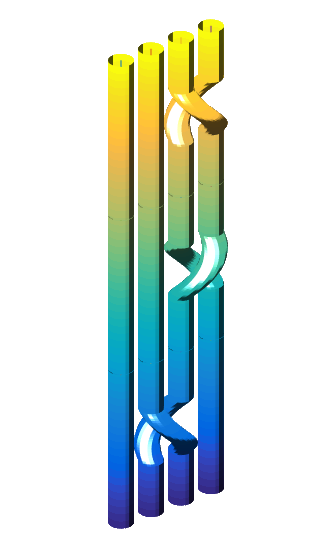
\includegraphics[width=4.5cm]{itrenzas/4c4.png}} 
   	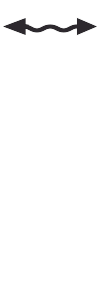
\includegraphics[width=1.2cm]{itrenzas/flechac.png}
   	\subfigure[$\beta2\beta1$]{
\includegraphics[width=5.5cm]{itrenzas/4c5.png}} 
   	\caption{No conmutatividad producto}
   	\label{grupo3} 
   \end{figure}

\begin{pro}  \textbf{Elemento neutro}.\label{prodneutro}\\
	Sea la trenza $\beta \in \mathscr{B}_{n}$. Se verifica:
	\begin{center}
		 $\beta 1_{n} \sim \beta \sim 1_{n} \beta$.
	\end{center}
	
	\begin{proof}	
		Es claro por la definición de n-trenza trivial $ 1_{n} $ (las cadenas de $ 1_{n} $ no tienen cruces luego no afectan a las cadenas de la trenza $ \beta $). 
	\end{proof}
\end{pro}

\begin{pro}  \textbf{Elemento inverso}.\label{prodinverso}\\
	Sea la trenza $\beta \in \mathscr{B}_{n}$. Existirá una trenza $\beta^{-1} \in \mathscr{B}_{n}$ verificando:
	\begin{center}
		$\beta \beta^{-1} \sim 1_{n} \sim \beta^{-1} \beta$.
	\end{center}
	A esta trenza $\beta^{-1}$ se le conoce como trenza inversa.
	
	\begin{proof} 
		Sea la trenza $\beta$ a la que notamos como $\beta = \sigma_{i_{1}}^{\pm 1} \sigma_{i_{2}}^{\pm 1} ... \sigma_{i_{m}}^{\pm 1}$\\

		 Construimos la trenza $\beta'$ a la que notamos como $\beta' = \sigma_{i_{m}}^{\mp 1} ...\sigma_{i_{2}}^{\mp 1} \sigma_{i_{1}}^{\mp 1}$. Veamos que esta trenza es la trenza inversa:
			\begin{center}
			 Por una parte, $\beta \beta'$ = $\sigma_{i_{1}}^{\pm 1} \sigma_{i_{2}}^{\pm 1} ... \sigma_{i_{m}}^{\pm 1} \sigma_{i_{m}}^{\mp 1} ...\sigma_{i_{2}}^{\mp 1} \sigma_{i_{1}}^{\mp 1}$ = $\sigma_{i_{1}}^{\pm 1} \sigma_{i_{2}}^{\pm 1} ... \sigma_{i_{m-1}}^{\pm 1} \sigma_{i_{m-1}}^{\mp 1} ...\sigma_{i_{2}}^{\mp 1} \sigma_{i_{1}}^{\mp 1}$ = $ 1_{n} $. Luego $\beta \beta' \sim 1_{n}$.\\
			\end{center}		 
			\begin{center}
			 Por otra parte, $ 1_{n} = \sigma_{i_{m}}^{\mp 1} \sigma_{i_{m}}^{\pm 1} = \sigma_{i_{m}}^{\mp 1} ...\sigma_{i_{2}}^{\mp 1} \sigma_{i_{2}}^{\pm 1} ... \sigma_{i_{m}}^{\pm 1} = \sigma_{i_{m}}^{\mp 1} ...\sigma_{i_{2}}^{\mp 1} \sigma_{i_{1}}^{\mp 1} \sigma_{i_{1}}^{\pm 1} \sigma_{i_{2}}^{\pm 1} ... \sigma_{i_{m}}^{\pm 1} = \beta' \beta$. Luego $1_{n} \sim \beta \beta'$.\\
			\end{center}
		 Por tanto $\beta' = \beta^{-1}$.\\
		 
		 Nota: estas igualdades son ciertas porque $\sigma_{i}^{\mp 1} \sigma_{i}^{\pm 1} = 1_{2}$ Se puede ver claro en la figura \ref{demo1}.
	      	\begin{figure}[h!]
			\centering
			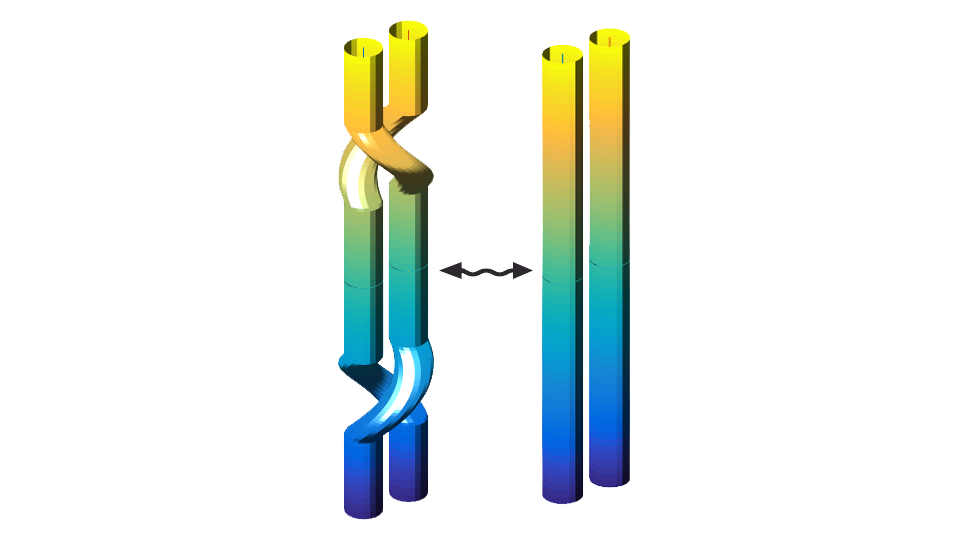
\includegraphics[width=7cm]{itrenzas/M1.png}
			\caption{Primer movimiento}
			\label{demo1} 
			\end{figure}	     
				
	\end{proof}
\end{pro}

En la figura \ref{grupo4} podemos ver un ejemplo de una trenza (a) y su trenza inversa (b). En la secuencia de trenzas (c)-(f) vemos que efectivamente su producto genera la trenza trivial.\\
   \begin{figure}[h!]
   	\centering
   	\subfigure[$\beta = \sigma4^{-1}\sigma1^{-1}\sigma2$]{
\includegraphics[width=5cm]{itrenzas/5c1.png}}
   	\subfigure[$\beta^{-1} = \sigma2^{-1}\sigma1\sigma4$]{
\includegraphics[width=4.7cm]{itrenzas/5c2.png}}
   	
   	\subfigure[$\beta\beta^{-1}$]{
\includegraphics[width=2cm]{itrenzas/5c3.png}}
   	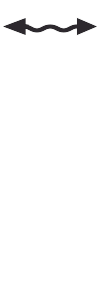
\includegraphics[width=1.2cm]{itrenzas/flechac.png}
   	\subfigure[$\beta\beta^{-1}$]{
\includegraphics[width=2cm]{itrenzas/5c4.png}} 
   	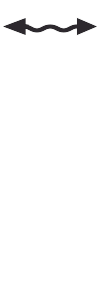
\includegraphics[width=1.2cm]{itrenzas/flechac.png}
   	\subfigure[$\beta\beta^{-1}$]{
\includegraphics[width=2cm]{itrenzas/5c5.png}} 
   	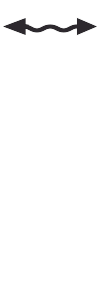
\includegraphics[width=1.2cm]{itrenzas/flechac.png}
   	\subfigure[$\beta\beta^{-1}$]{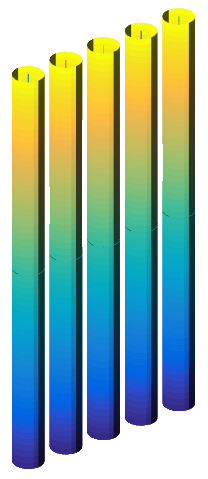
\includegraphics[width=2cm]{itrenzas/5c6.png}} 
   	\caption{Trenzas inversas}
   	\label{grupo4} 
   \end{figure}

\begin{teo}
	El conjunto ${B}_{n}$, dotado del producto de trenzas, es un grupo. El grupo se conoce como el grupo de n-trenzas o el \textbf{grupo de n-trenzas de Artin}. 
	\begin{proof} Sea la trenza $\beta \in \mathscr{B}_{n}$, denotamos su clase de equivalencia como $[\beta] \in {B}_{n}$. Veamos que  ${B}_{n}$ es un grupo: \\
		\begin{enumerate}
			\item 
			Por la proposición \ref{prod1} sabemos que el producto de trenzas está bien definido: Sean $[\beta1],[\beta2] \in {B}_{n}$, se tiene que $[\beta1][\beta2] = [\beta1\beta2] $
			\item 
			Por la proposición \ref{prodaso} sabemos que el producto de trenzas es asociativo.
			\item 
			Por la proposición \ref{prodneutro} sabemos que la n-trenza trivial es el elemento identidad para el producto de trenzas.
			\item 
			Por la proposición \ref{prodinverso} sabemos que el elemento inverso de  $[\beta] \in {B}_{n}$ es $[\beta^{-1}]$, luego  $[\beta]^{-1}$ =  $[\beta^{-1}]$.
		\end{enumerate}
	\end{proof}
\end{teo}

\bigskip
	\subsection{Trenzas equivalentes:}\label{trenzasequi}
	
	Hemos definido $\mathscr{B}_{n}$ como el conjunto de todas las n-trenzas, siendo estas n-trenzas representadas por palabras. En concreto si tenemos la trenza $\beta \in \mathscr{B}_{n}$, que consta de m-cruces, la podremos representar como:
    \begin{center}
    	$\beta = \sigma_{i_{1}}^{\pm 1} \sigma_{i_{2}}^{\pm 1} ... \sigma_{i_{m}}^{\pm 1} $, 1 $\le i_{1}, i_{2},..,i_{m} \le$ n-1.
    \end{center}
	
	Además, hemos visto que el conjunto $B_{n} $ = $\mathscr{B}_{n}$/$ \sim $, de todas las n-trenzas no equivalentes entre sí, tiene estructura de grupo al dotarle del producto de trenzas.\\
	
	En esta sección vamos a ver cuáles son los movimientos que nos permitirán estudiar la equivalencia de dos n-trenzas y posteriormente vamos a reflejar estos movimientos como el conjunto de relaciones que representan al conjunto $B_{n}$.\\
	
	Para analizar cuándo dos trenzas son equivalentes tendremos que ver cuándo las palabras que representan a dichas trenzas son equivalentes. Dos palabras serán equivalentes si y sólo si podemos pasar de una palabra a otra mediante un secuencia de estos tres movimientos:
	\begin{enumerate}
		\item \underline{Primer movimiento - M1:} \\
		Podemos añadir o eliminar $\sigma_{i}\sigma_{i}^{-1}$ o $\sigma_{i}^{-1}\sigma_{i}$ en cualquier palabra. Es claro que la palabra inicial y la palabra final representan a la misma trenza. Podemos verlo en la figura \ref{tren6}.
		\begin{figure}[h!]
			\centering
			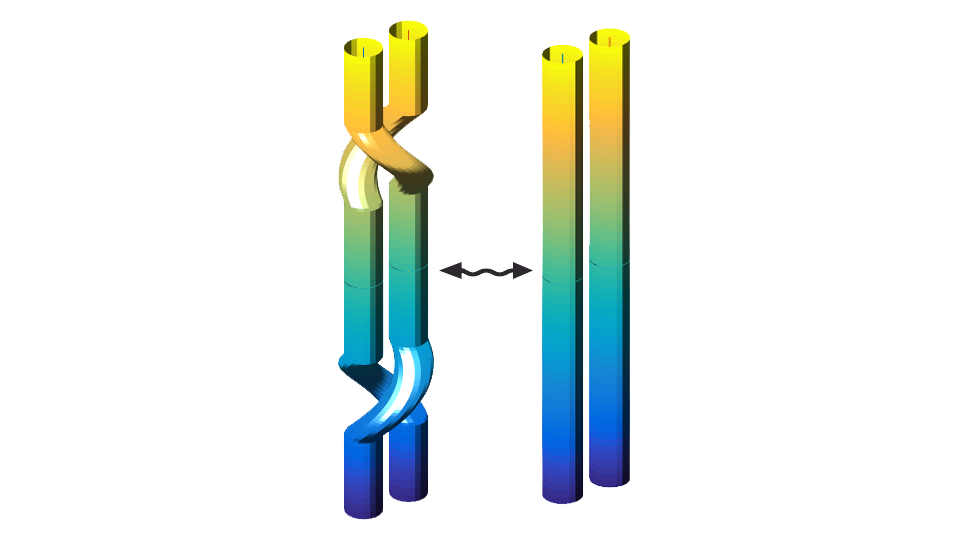
\includegraphics[width=5.1cm]{itrenzas/M1.png}
			\caption{Primer movimiento.}
			\label{tren6} 
		\end{figure}
		
		\item \underline{Segundo movimiento - M2:} \\
		Las palabras $\sigma_{i} \sigma_{i+1} \sigma_{i}$ y $\sigma_{i+1} \sigma_{i} \sigma_{i+1}$ son equivalentes (o bien con cruces negativos). Se puede ver en la figura \ref{tren7}.
		\begin{figure}[h!]
			\centering
			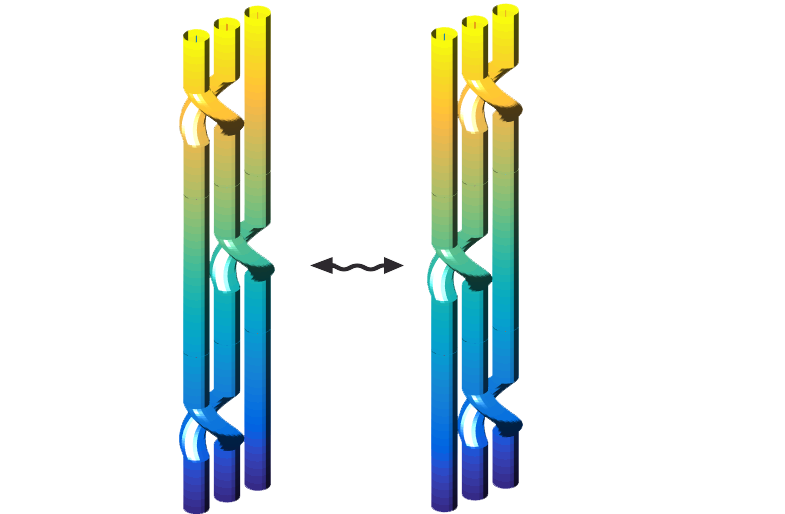
\includegraphics[width=8cm]{itrenzas/M2.png}
			\caption{Segundo movimiento.}
			\label{tren7} 
		\end{figure}
		
		
		\item \underline{Tercer movimiento - M3:} \\
		Las palabras $\sigma_{i} \sigma_{j}$ y $\sigma_{j} \sigma_{i}$ son equivalentes si se verifica que $|i-j| > 1$ (o bien con cruces negativos). Se ve claro en la figura \ref{tren8}.
		\begin{figure}[h!]
			\centering
			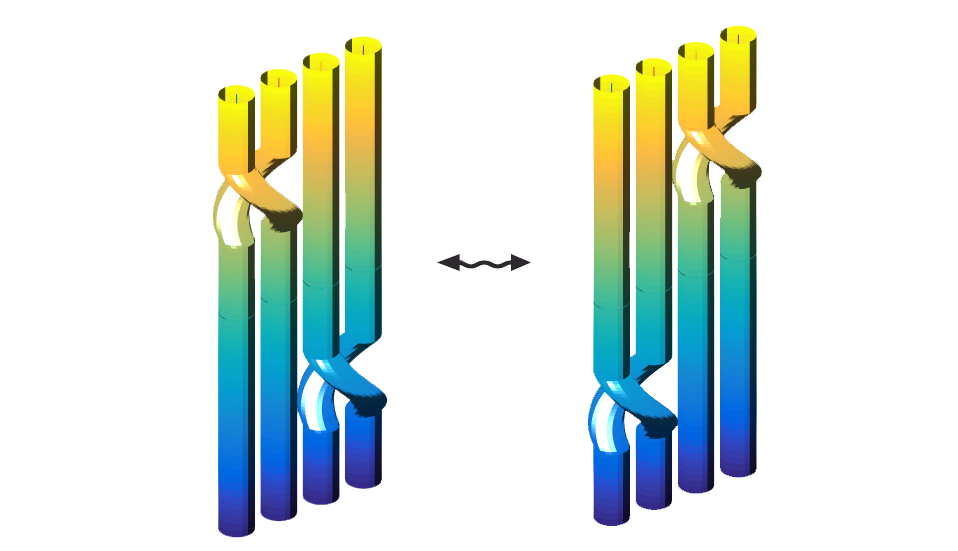
\includegraphics[width=10cm]{itrenzas/M3.png}
			\caption{Tercer movimiento.}
			\label{tren8} 
		\end{figure}
		
	\end{enumerate}
	En la figura \ref{tren9} podemos ver los movimientos que nos demuestran que dos trenzas dadas más complejas son equivalentes. \\
	Partimos de la trenza $\sigma3^{-1}\sigma1\sigma2^{-1}\sigma3^{-1}$ y aplicamos M3 a los dos primeros cruces obteniendo la trenza $\sigma1\sigma3^{-1}\sigma2^{-1}\sigma3^{-1}$ que vemos en la segunda imagen. \\
	Por último, aplicamos el movimiento M2 a los tres últimos cruces obteniendo la trenza $\sigma1\sigma2^{-1}\sigma3^{-1}\sigma2^{-1}$ que vemos en la última imagen.\\
	\begin{figure}[h!]
		\centering
		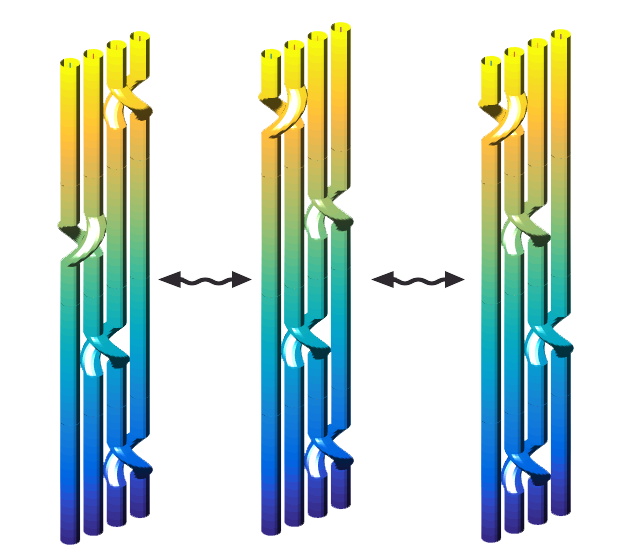
\includegraphics[width=10cm]{itrenzas/movi.png}
		\caption{Trenzas equivalentes.}
		\label{tren9} 
	\end{figure}
	
	\begin{teo}	    \label{teoBn}
	    Defino las relaciones:
	    \begin{enumerate}
	    	\item $ \sigma_{i+1}\sigma_{i}\sigma_{i+1} =\sigma_{i}\sigma_{i+1}\sigma_{i} $ siendo $i=2,..,n-2 $ \label{rel1}
	    	\item $ \sigma_{i}\sigma_{j}=\sigma_{j}\sigma_{i} $ siendo $1 \le i < j \le n-1 $, $j-i \geq 2$	 \label{rel2}   	
	    \end{enumerate}
	    El grupo $B_{n}$ tiene la siguiente representación:
        \begin{center}
			$B_{n} = <\sigma1, \sigma2,..,\sigma_{n-1} /$ las relaciones \ref{rel1} y \ref{rel2} se verifican$>$
        \end{center}
	   
	\end{teo}
	
	A partir de estas relaciones de equivalencia base podremos construir nuevas relaciones de equivalencia. Vamos a mostrar algunas relaciones de equivalencia que usaremos posteriormente:
	\begin{enumerate}
		\item $ \sigma_{i+1}\sigma_{i}\sigma_{i+1}^{-1} =\sigma_{i}^{-1}\sigma_{i+1}\sigma_{i} $ siendo $i=2,..,n-2 $		
		\item $ \sigma_{i+1}\sigma_{i}^{-1}\sigma_{i+1}^{-1} =\sigma_{i}^{-1}\sigma_{i+1}^{-1}\sigma_{i} $ siendo $i=2,..,n-2 $
	\end{enumerate}
	
    \underline{	Demostración:}
    \begin{enumerate}
    	\item $ \sigma_{i+1}\sigma_{i}\sigma_{i+1}^{-1} = \sigma_{i}^{-1}\sigma_{i}\sigma_{i+1}\sigma_{i}\sigma_{i+1}^{-1} = \sigma_{i}^{-1}\sigma_{i+1}\sigma_{i}\sigma_{i+1}\sigma_{i+1}^{-1} =  \sigma_{i}^{-1}\sigma_{i+1}\sigma_{i} $ 		
    	\item $ \sigma_{i+1}\sigma_{i}^{-1}\sigma_{i+1}^{-1} = \sigma_{i+1}\sigma_{i}^{-1}\sigma_{i+1}^{-1}\sigma_{i}^{-1}\sigma_{i}=\sigma_{i+1}\sigma_{i+1}^{-1}\sigma_{i}^{-1}\sigma_{i+1}^{-1}\sigma_{i} = \sigma_{i}^{-1}\sigma_{i+1}^{-1}\sigma_{i}$
    \end{enumerate}
	

	En la figura \ref{tren14} podemos visualizar las equivalencias.\\
	\begin{figure}[h!]
		\centering
		
\includegraphics[width=3cm]{itrenzas/6c1.png}
		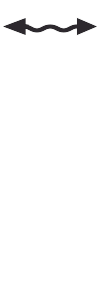
\includegraphics[width=0.7cm]{itrenzas/flechac.png}
		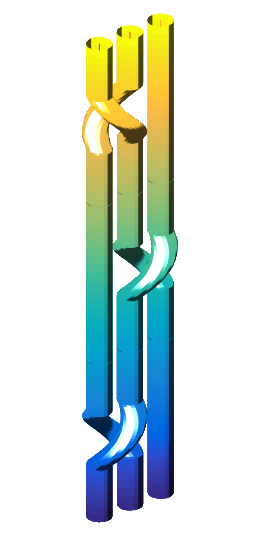
\includegraphics[width=2.6cm]{itrenzas/6c2.png}
		\space	
		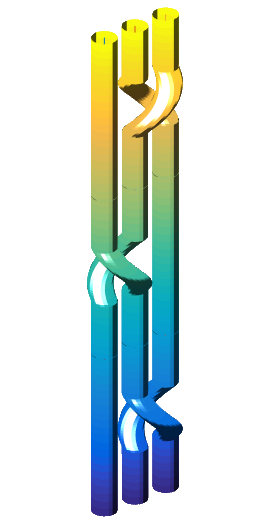
\includegraphics[width=2.7cm]{itrenzas/6c3.png}
		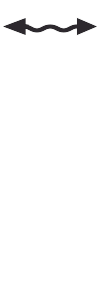
\includegraphics[width=0.7cm]{itrenzas/flechac.png}
		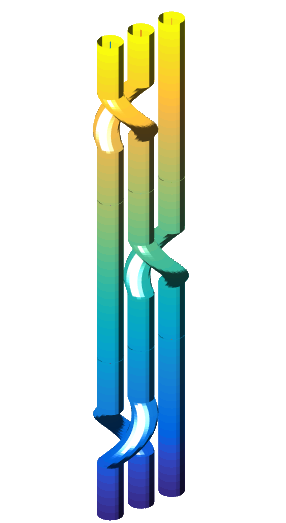
\includegraphics[width=2.9cm]{itrenzas/6c4.png}
		\caption{Trenzas equivalentes.}
		\label{tren14} 
	\end{figure}


\newpage
\begin{center}
	\subsection{Trenzas Markov-equivalentes:}\label{Markov}
\end{center}
Es claro que si tenemos dos trenzas que son equivalentes, sus trenzas cerradas nos darán nudos que serán equivalentes. Pero...¿puede darse el caso de tener dos trenzas no sean equivalentes y que sus trenzas cerradas sí lo sean? Veamos, mediante el ejemplo de la figura \ref{tren10} que sí es posible: las trenzas de partida no son equivalentes (tenemos distinto número de cadenas), sin embargo sus trenzas cerradas sí lo son. Lo demostraremos en la figura \ref{tren13}.\\
\begin{figure}[h!]
	\centering
	
\includegraphics[width=3cm]{itrenzas/t1pro.png}
	
\includegraphics[width=2.5cm]{itrenzas/t2pro.png}
	
	
\includegraphics[width=3.5cm]{itrenzas/t1probien.png}
	
\includegraphics[width=3.5cm]{itrenzas/t2probien.png}
	\caption{Trenzas Markov-equivalentes.}
	\label{tren10} 
\end{figure}

\underline{\textit{Definición:}}\\
Se dice que dos trenzas son \textbf{Markov-equivalentes} si sus cierres producen el mismo enlace. En este caso tendremos que los nudos representados por las trenzas son equivalentes. \\

\begin{teo} \textbf{Teorema de Markov.} \label{teoMarkov}\\
	Dos trenzas son Markov-equivalentes si y solo si podemos pasar de una trenza a otra mediante una secuencia de las tres operaciones que hemos visto en la subsección \ref{trenzasequi} y los movimientos de Markov.
\end{teo}

Veamos los movimientos de Markov:
\begin{enumerate}
	\item \underline{Conjugación - Mv1:} \\
	Las palabras $\beta$ y $\sigma_{i} \beta \sigma_{i}^{-1}$ (o bien  $\sigma_{i}^{-1} \beta \sigma_{i}$) generan trenzas cerradas equivalentes. Se puede ver en la figura \ref{tren11}.
	\begin{figure}[h!]
		\centering
		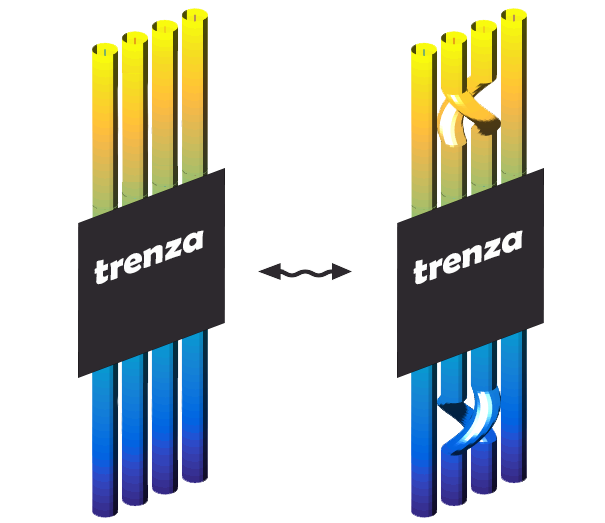
\includegraphics[width=8cm]{itrenzas/M4.png}
		\caption{Conjugación Markov.}
		\label{tren11} 
	\end{figure}
	
	\item \underline{Estabilización - Mv2:} \\
	Esta operación nos permite modificar el número de cadenas de las trenzas. 
	Sea la palabra $\beta$ de n cadenas. Esta palabra genera una trenza cerrada equivalente a $\beta \sigma_{n}$ o bien $\sigma_{n} \beta $. Se puede ver en la figura \ref{tren12}.
	\begin{figure}[h!]
		\centering
		\includegraphics[width=7cm]{itrenzas/M5.png}
		\caption{Estabilización Markov.}
		\label{tren12} 
	\end{figure}
	
\end{enumerate}

Podemos ver un ejemplo de dos trenzas Markov-equivalentes en la figura \ref{tren13}.
\begin{figure}[h!]
	\centering
	\subfigure[$\sigma2^{-1}\sigma1\sigma2^{-1}\sigma1\sigma3$]{\includegraphics[width=3.5cm]{itrenzas/t1probien.png}}
	\subfigure[Mv2]{\includegraphics[width=1cm]{itrenzas/flechac.png}}
	\subfigure[$\sigma2^{-1}\sigma1\sigma2^{-1}\sigma1$]{\includegraphics[width=3.5cm]{itrenzas/t3probien.png}}
	\subfigure[Mv1]{\includegraphics[width=1cm]{itrenzas/flechac.png}}
	\subfigure[$\sigma1\sigma2^{-1}\sigma1$ $\sigma2^{-1}\sigma1\sigma1^{-1}$]{\includegraphics[width=2.4cm]{itrenzas/t4probien.png}}
	\subfigure[M1]{\includegraphics[width=1cm]{itrenzas/flechac.png}}
	\subfigure[$\sigma1\sigma2^{-1}\sigma1\sigma2^{-1}$]{\includegraphics[width=3.5cm]{itrenzas/t2probien.png}}
	\caption{Trenzas Markov-equivalentes.}
	\label{tren13} 
\end{figure}
